\documentclass[]{article}
\usepackage{lmodern}
\usepackage{amssymb,amsmath}
\usepackage{ifxetex,ifluatex}
\usepackage{fixltx2e} % provides \textsubscript
\ifnum 0\ifxetex 1\fi\ifluatex 1\fi=0 % if pdftex
  \usepackage[T1]{fontenc}
  \usepackage[utf8]{inputenc}
\else % if luatex or xelatex
  \ifxetex
    \usepackage{mathspec}
  \else
    \usepackage{fontspec}
  \fi
  \defaultfontfeatures{Ligatures=TeX,Scale=MatchLowercase}
\fi
% use upquote if available, for straight quotes in verbatim environments
\IfFileExists{upquote.sty}{\usepackage{upquote}}{}
% use microtype if available
\IfFileExists{microtype.sty}{%
\usepackage{microtype}
\UseMicrotypeSet[protrusion]{basicmath} % disable protrusion for tt fonts
}{}
\usepackage[margin=1in]{geometry}
\usepackage{hyperref}
\hypersetup{unicode=true,
            pdftitle={Eksploracja Masywnych Danych - Analiza danych},
            pdfauthor={Kajetan Zimniak \& Bartosz Górka},
            pdfborder={0 0 0},
            breaklinks=true}
\urlstyle{same}  % don't use monospace font for urls
\usepackage{color}
\usepackage{fancyvrb}
\newcommand{\VerbBar}{|}
\newcommand{\VERB}{\Verb[commandchars=\\\{\}]}
\DefineVerbatimEnvironment{Highlighting}{Verbatim}{commandchars=\\\{\}}
% Add ',fontsize=\small' for more characters per line
\usepackage{framed}
\definecolor{shadecolor}{RGB}{248,248,248}
\newenvironment{Shaded}{\begin{snugshade}}{\end{snugshade}}
\newcommand{\AlertTok}[1]{\textcolor[rgb]{0.94,0.16,0.16}{#1}}
\newcommand{\AnnotationTok}[1]{\textcolor[rgb]{0.56,0.35,0.01}{\textbf{\textit{#1}}}}
\newcommand{\AttributeTok}[1]{\textcolor[rgb]{0.77,0.63,0.00}{#1}}
\newcommand{\BaseNTok}[1]{\textcolor[rgb]{0.00,0.00,0.81}{#1}}
\newcommand{\BuiltInTok}[1]{#1}
\newcommand{\CharTok}[1]{\textcolor[rgb]{0.31,0.60,0.02}{#1}}
\newcommand{\CommentTok}[1]{\textcolor[rgb]{0.56,0.35,0.01}{\textit{#1}}}
\newcommand{\CommentVarTok}[1]{\textcolor[rgb]{0.56,0.35,0.01}{\textbf{\textit{#1}}}}
\newcommand{\ConstantTok}[1]{\textcolor[rgb]{0.00,0.00,0.00}{#1}}
\newcommand{\ControlFlowTok}[1]{\textcolor[rgb]{0.13,0.29,0.53}{\textbf{#1}}}
\newcommand{\DataTypeTok}[1]{\textcolor[rgb]{0.13,0.29,0.53}{#1}}
\newcommand{\DecValTok}[1]{\textcolor[rgb]{0.00,0.00,0.81}{#1}}
\newcommand{\DocumentationTok}[1]{\textcolor[rgb]{0.56,0.35,0.01}{\textbf{\textit{#1}}}}
\newcommand{\ErrorTok}[1]{\textcolor[rgb]{0.64,0.00,0.00}{\textbf{#1}}}
\newcommand{\ExtensionTok}[1]{#1}
\newcommand{\FloatTok}[1]{\textcolor[rgb]{0.00,0.00,0.81}{#1}}
\newcommand{\FunctionTok}[1]{\textcolor[rgb]{0.00,0.00,0.00}{#1}}
\newcommand{\ImportTok}[1]{#1}
\newcommand{\InformationTok}[1]{\textcolor[rgb]{0.56,0.35,0.01}{\textbf{\textit{#1}}}}
\newcommand{\KeywordTok}[1]{\textcolor[rgb]{0.13,0.29,0.53}{\textbf{#1}}}
\newcommand{\NormalTok}[1]{#1}
\newcommand{\OperatorTok}[1]{\textcolor[rgb]{0.81,0.36,0.00}{\textbf{#1}}}
\newcommand{\OtherTok}[1]{\textcolor[rgb]{0.56,0.35,0.01}{#1}}
\newcommand{\PreprocessorTok}[1]{\textcolor[rgb]{0.56,0.35,0.01}{\textit{#1}}}
\newcommand{\RegionMarkerTok}[1]{#1}
\newcommand{\SpecialCharTok}[1]{\textcolor[rgb]{0.00,0.00,0.00}{#1}}
\newcommand{\SpecialStringTok}[1]{\textcolor[rgb]{0.31,0.60,0.02}{#1}}
\newcommand{\StringTok}[1]{\textcolor[rgb]{0.31,0.60,0.02}{#1}}
\newcommand{\VariableTok}[1]{\textcolor[rgb]{0.00,0.00,0.00}{#1}}
\newcommand{\VerbatimStringTok}[1]{\textcolor[rgb]{0.31,0.60,0.02}{#1}}
\newcommand{\WarningTok}[1]{\textcolor[rgb]{0.56,0.35,0.01}{\textbf{\textit{#1}}}}
\usepackage{longtable,booktabs}
\usepackage{graphicx,grffile}
\makeatletter
\def\maxwidth{\ifdim\Gin@nat@width>\linewidth\linewidth\else\Gin@nat@width\fi}
\def\maxheight{\ifdim\Gin@nat@height>\textheight\textheight\else\Gin@nat@height\fi}
\makeatother
% Scale images if necessary, so that they will not overflow the page
% margins by default, and it is still possible to overwrite the defaults
% using explicit options in \includegraphics[width, height, ...]{}
\setkeys{Gin}{width=\maxwidth,height=\maxheight,keepaspectratio}
\IfFileExists{parskip.sty}{%
\usepackage{parskip}
}{% else
\setlength{\parindent}{0pt}
\setlength{\parskip}{6pt plus 2pt minus 1pt}
}
\setlength{\emergencystretch}{3em}  % prevent overfull lines
\providecommand{\tightlist}{%
  \setlength{\itemsep}{0pt}\setlength{\parskip}{0pt}}
\setcounter{secnumdepth}{0}
% Redefines (sub)paragraphs to behave more like sections
\ifx\paragraph\undefined\else
\let\oldparagraph\paragraph
\renewcommand{\paragraph}[1]{\oldparagraph{#1}\mbox{}}
\fi
\ifx\subparagraph\undefined\else
\let\oldsubparagraph\subparagraph
\renewcommand{\subparagraph}[1]{\oldsubparagraph{#1}\mbox{}}
\fi

%%% Use protect on footnotes to avoid problems with footnotes in titles
\let\rmarkdownfootnote\footnote%
\def\footnote{\protect\rmarkdownfootnote}

%%% Change title format to be more compact
\usepackage{titling}

% Create subtitle command for use in maketitle
\providecommand{\subtitle}[1]{
  \posttitle{
    \begin{center}\large#1\end{center}
    }
}

\setlength{\droptitle}{-2em}

  \title{Eksploracja Masywnych Danych - Analiza danych}
    \pretitle{\vspace{\droptitle}\centering\huge}
  \posttitle{\par}
    \author{Kajetan Zimniak \& Bartosz Górka}
    \preauthor{\centering\large\emph}
  \postauthor{\par}
      \predate{\centering\large\emph}
  \postdate{\par}
    \date{01 November, 2019}


\begin{document}
\maketitle

{
\setcounter{tocdepth}{2}
\tableofcontents
}
\hypertarget{podsumowanie-analizy}{%
\section{Podsumowanie analizy}\label{podsumowanie-analizy}}

TODO: Podsumowanie na koniec

\hypertarget{wykorzystane-biblioteki}{%
\section{Wykorzystane biblioteki}\label{wykorzystane-biblioteki}}

\begin{itemize}
\tightlist
\item
  \texttt{knitr}
\item
  \texttt{dplyr}
\item
  \texttt{tidyverse}
\item
  \texttt{ggplot2}
\item
  \texttt{gridExtra}
\item
  \texttt{imputeTS}
\item
  \texttt{corrplot}
\item
  \texttt{reshape2}
\end{itemize}

\hypertarget{ustawienie-ziarna-generatora}{%
\section{Ustawienie ziarna
generatora}\label{ustawienie-ziarna-generatora}}

Celem zapewnienia powtarzalności operacji losowania, a co za tym idzie
powtarzalności wyników przy każdym uruchomieniu raportu na tych samych
danych zastosowano ziarno generatora o wartości \texttt{102019}.

\begin{Shaded}
\begin{Highlighting}[]
\KeywordTok{set.seed}\NormalTok{(}\DecValTok{102019}\NormalTok{)}
\end{Highlighting}
\end{Shaded}

\hypertarget{charakterystyka-obserwacji---zastosowane-atrybuty}{%
\section{Charakterystyka obserwacji - zastosowane
atrybuty}\label{charakterystyka-obserwacji---zastosowane-atrybuty}}

W ramach analizy mamy do czynienia z obserwacjami opisanymi za pomocą
następujących atrybutów:

\begin{itemize}
\tightlist
\item
  \textbf{length}: długość złowionego śledzia {[}cm{]}
\item
  \textbf{cfin1}: dostępność planktonu {[}zagęszczenie \emph{Calanus
  finmarchicus} gat. 1{]}
\item
  \textbf{cfin2}: dostępność planktonu {[}zagęszczenie \emph{Calanus
  finmarchicus} gat. 2{]};
\item
  \textbf{chel1}: dostępność planktonu {[}zagęszczenie \emph{Calanus
  helgolandicus} gat. 1{]};
\item
  \textbf{chel2}: dostępność planktonu {[}zagęszczenie \emph{Calanus
  helgolandicus} gat. 2{]};
\item
  \textbf{lcop1}: dostępność planktonu {[}zagęszczenie \emph{widłonogów}
  gat. 1{]};
\item
  \textbf{lcop2}: dostępność planktonu {[}zagęszczenie \emph{widłonogów}
  gat. 2{]};
\item
  \textbf{fbar}: natężenie połowów w regionie {[}ułamek pozostawionego
  narybku{]};
\item
  \textbf{recr}: roczny narybek {[}liczba śledzi{]};
\item
  \textbf{cumf}: łączne roczne natężenie połowów w regionie {[}ułamek
  pozostawionego narybku{]};
\item
  \textbf{totaln}: łączna liczba ryb złowionych w ramach połowu
  {[}liczba śledzi{]};
\item
  \textbf{sst}: temperatura przy powierzchni wody {[}°C{]};
\item
  \textbf{sal}: poziom zasolenia wody {[}Knudsen ppt{]};
\item
  \textbf{xmonth}: miesiąc połowu {[}numer miesiąca{]};
\item
  \textbf{nao}: oscylacja północnoatlantycka {[}mb{]}.
\end{itemize}

\hypertarget{wczytanie-danych-z-pliku}{%
\section{Wczytanie danych z pliku}\label{wczytanie-danych-z-pliku}}

Dane zamieszczone na stronie przedmiotu w postaci pliku CSV pobieramy
wyłącznie w sytuacji braku pliku w katalogu roboczym. Pozwala to nam na
ograniczenie niepotrzebnego transferu danych, jeżeli plik już istnieje.

\begin{Shaded}
\begin{Highlighting}[]
\NormalTok{file_name =}\StringTok{ "sledzie.csv"}
\NormalTok{source_url =}\StringTok{ "http://www.cs.put.poznan.pl/alabijak/emd/projekt/sledzie.csv"}

\ControlFlowTok{if}\NormalTok{ (}\OperatorTok{!}\KeywordTok{file.exists}\NormalTok{(file_name)) \{}
  \KeywordTok{download.file}\NormalTok{(source_url, }\DataTypeTok{destfile =}\NormalTok{ file_name, }\DataTypeTok{method =} \StringTok{"wget"}\NormalTok{)}
\NormalTok{\}}
\end{Highlighting}
\end{Shaded}

Po ewentualnym pobraniu wczytujemy dane do pamięci.

\begin{Shaded}
\begin{Highlighting}[]
\KeywordTok{library}\NormalTok{(}\StringTok{'knitr'}\NormalTok{)}
\KeywordTok{library}\NormalTok{(}\StringTok{'dplyr'}\NormalTok{)}
\KeywordTok{library}\NormalTok{(}\StringTok{'tidyverse'}\NormalTok{)}

\NormalTok{content =}
\StringTok{  }\NormalTok{file_name }\OperatorTok
\StringTok{  }\KeywordTok{read_csv}\NormalTok{(}\DataTypeTok{col_names =} \OtherTok{TRUE}\NormalTok{, }\DataTypeTok{na =} \KeywordTok{c}\NormalTok{(}\StringTok{""}\NormalTok{, }\StringTok{"NA"}\NormalTok{, }\StringTok{"?"}\NormalTok{)) }\OperatorTok
\StringTok{  }\KeywordTok{select}\NormalTok{(}\OperatorTok{-}\DecValTok{1}\NormalTok{)}

\NormalTok{content[}\DecValTok{0}\OperatorTok{:}\DecValTok{11}\NormalTok{] }\OperatorTok
\StringTok{  }\KeywordTok{head}\NormalTok{(}\DataTypeTok{n =} \DecValTok{5}\NormalTok{) }\OperatorTok
\StringTok{  }\KeywordTok{kable}\NormalTok{(}\DataTypeTok{align =} \StringTok{'c'}\NormalTok{, }\DataTypeTok{caption =} \StringTok{'Wybrane pomiary'}\NormalTok{)}
\end{Highlighting}
\end{Shaded}

\begin{longtable}[]{@{}ccccccccccc@{}}
\caption{Wybrane pomiary}\tabularnewline
\toprule
length & cfin1 & cfin2 & chel1 & chel2 & lcop1 & lcop2 & fbar & recr &
cumf & totaln\tabularnewline
\midrule
\endfirsthead
\toprule
length & cfin1 & cfin2 & chel1 & chel2 & lcop1 & lcop2 & fbar & recr &
cumf & totaln\tabularnewline
\midrule
\endhead
23.0 & 0.02778 & 0.27785 & 2.46875 & NA & 2.54787 & 26.35881 & 0.356 &
482831 & 0.3059879 & 267380.8\tabularnewline
22.5 & 0.02778 & 0.27785 & 2.46875 & 21.43548 & 2.54787 & 26.35881 &
0.356 & 482831 & 0.3059879 & 267380.8\tabularnewline
25.0 & 0.02778 & 0.27785 & 2.46875 & 21.43548 & 2.54787 & 26.35881 &
0.356 & 482831 & 0.3059879 & 267380.8\tabularnewline
25.5 & 0.02778 & 0.27785 & 2.46875 & 21.43548 & 2.54787 & 26.35881 &
0.356 & 482831 & 0.3059879 & 267380.8\tabularnewline
24.0 & 0.02778 & 0.27785 & 2.46875 & 21.43548 & 2.54787 & 26.35881 &
0.356 & 482831 & 0.3059879 & 267380.8\tabularnewline
\bottomrule
\end{longtable}

Oryginalnie zbiór posiada znaki \texttt{?} jako oznaczenie wartości
pustej (brakującej). Dzięki wykorzystaniu parametru \texttt{na} podczas
wywołania funkcji \texttt{read\_csv} możemy zastąpić znak \texttt{?}
poprawnym oznaczeniem braku wartości \texttt{NA}. W tabeli
\texttt{Wybrane\ pomiary} zaprezentowano pierwsze pięć obserwacji.

\hypertarget{podstawowe-statystyki-zbioru-danych}{%
\section{Podstawowe statystyki zbioru
danych}\label{podstawowe-statystyki-zbioru-danych}}

\begin{Shaded}
\begin{Highlighting}[]
\NormalTok{total_records =}\StringTok{ }\KeywordTok{count}\NormalTok{(content)}
\NormalTok{total_records_without_na_values =}\StringTok{ }\KeywordTok{count}\NormalTok{(}\KeywordTok{na.omit}\NormalTok{(content))}
\end{Highlighting}
\end{Shaded}

W zbiorze danych mamy do czynienia z 52582 obserwacjami opisanych za
pomocą 15 atrybutów. W całym zbiorze mamy do czynienia z 42488
obserwacjami bez wartości pustych co stanowi 81 procent całego zbioru.

\hypertarget{statystyka-parametruxf3w-obserwacji}{%
\subsection{Statystyka parametrów
obserwacji}\label{statystyka-parametruxf3w-obserwacji}}

\begin{Shaded}
\begin{Highlighting}[]
\NormalTok{content }\OperatorTok
\StringTok{  }\KeywordTok{summary}\NormalTok{() }\OperatorTok
\StringTok{  }\KeywordTok{kable}\NormalTok{(}\DataTypeTok{align =} \StringTok{'c'}\NormalTok{, }\DataTypeTok{caption =} \StringTok{'Statystyka zbioru danych'}\NormalTok{)}
\end{Highlighting}
\end{Shaded}

\begin{longtable}[]{@{}lccccccccccccccc@{}}
\caption{Statystyka zbioru danych}\tabularnewline
\toprule
& length & cfin1 & cfin2 & chel1 & chel2 & lcop1 & lcop2 & fbar & recr &
cumf & totaln & sst & sal & xmonth & nao\tabularnewline
\midrule
\endfirsthead
\toprule
& length & cfin1 & cfin2 & chel1 & chel2 & lcop1 & lcop2 & fbar & recr &
cumf & totaln & sst & sal & xmonth & nao\tabularnewline
\midrule
\endhead
& Min. :19.0 & Min. : 0.0000 & Min. : 0.0000 & Min. : 0.000 & Min. :
5.238 & Min. : 0.3074 & Min. : 7.849 & Min. :0.0680 & Min. : 140515 &
Min. :0.06833 & Min. : 144137 & Min. :12.77 & Min. :35.40 & Min. : 1.000
& Min. :-4.89000\tabularnewline
& 1st Qu.:24.0 & 1st Qu.: 0.0000 & 1st Qu.: 0.2778 & 1st Qu.: 2.469 &
1st Qu.:13.427 & 1st Qu.: 2.5479 & 1st Qu.:17.808 & 1st Qu.:0.2270 & 1st
Qu.: 360061 & 1st Qu.:0.14809 & 1st Qu.: 306068 & 1st Qu.:13.60 & 1st
Qu.:35.51 & 1st Qu.: 5.000 & 1st Qu.:-1.89000\tabularnewline
& Median :25.5 & Median : 0.1111 & Median : 0.7012 & Median : 5.750 &
Median :21.673 & Median : 7.0000 & Median :24.859 & Median :0.3320 &
Median : 421391 & Median :0.23191 & Median : 539558 & Median :13.86 &
Median :35.51 & Median : 8.000 & Median : 0.20000\tabularnewline
& Mean :25.3 & Mean : 0.4458 & Mean : 2.0248 & Mean :10.006 & Mean
:21.221 & Mean : 12.8108 & Mean :28.419 & Mean :0.3304 & Mean : 520366 &
Mean :0.22981 & Mean : 514973 & Mean :13.87 & Mean :35.51 & Mean : 7.258
& Mean :-0.09236\tabularnewline
& 3rd Qu.:26.5 & 3rd Qu.: 0.3333 & 3rd Qu.: 1.7936 & 3rd Qu.:11.500 &
3rd Qu.:27.193 & 3rd Qu.: 21.2315 & 3rd Qu.:37.232 & 3rd Qu.:0.4560 &
3rd Qu.: 724151 & 3rd Qu.:0.29803 & 3rd Qu.: 730351 & 3rd Qu.:14.16 &
3rd Qu.:35.52 & 3rd Qu.: 9.000 & 3rd Qu.: 1.63000\tabularnewline
& Max. :32.5 & Max. :37.6667 & Max. :19.3958 & Max. :75.000 & Max.
:57.706 & Max. :115.5833 & Max. :68.736 & Max. :0.8490 & Max. :1565890 &
Max. :0.39801 & Max. :1015595 & Max. :14.73 & Max. :35.61 & Max. :12.000
& Max. : 5.08000\tabularnewline
& NA & NA's :1581 & NA's :1536 & NA's :1555 & NA's :1556 & NA's :1653 &
NA's :1591 & NA & NA & NA & NA & NA's :1584 & NA & NA &
NA\tabularnewline
\bottomrule
\end{longtable}

TODO: Poprawić tabelkę, nie mieści się na stronie PDF

\hypertarget{rozkux142ad-wartoux15bci-cech}{%
\subsection{Rozkład wartości cech}\label{rozkux142ad-wartoux15bci-cech}}

\begin{Shaded}
\begin{Highlighting}[]
\KeywordTok{library}\NormalTok{(}\StringTok{'ggplot2'}\NormalTok{)}
\KeywordTok{library}\NormalTok{(}\StringTok{'gridExtra'}\NormalTok{)}

\KeywordTok{ggplot}\NormalTok{(content, }\KeywordTok{aes}\NormalTok{(}\DataTypeTok{x =}\NormalTok{ length)) }\OperatorTok{+}\StringTok{ }\KeywordTok{geom_histogram}\NormalTok{(}\DataTypeTok{binwidth =} \FloatTok{0.25}\NormalTok{) }\OperatorTok{+}\StringTok{ }
\StringTok{  }\KeywordTok{theme_bw}\NormalTok{() }\OperatorTok{+}\StringTok{ }\KeywordTok{ggtitle}\NormalTok{(}\StringTok{'Długość złowionego śledzia [cm]'}\NormalTok{) }\OperatorTok{+}\StringTok{ }
\StringTok{  }\KeywordTok{xlab}\NormalTok{(}\KeywordTok{sprintf}\NormalTok{(}\StringTok{'Długość [cm]'}\NormalTok{)) }\OperatorTok{+}\StringTok{ }\KeywordTok{ylab}\NormalTok{(}\StringTok{'Liczba obserwacji'}\NormalTok{)}
\end{Highlighting}
\end{Shaded}

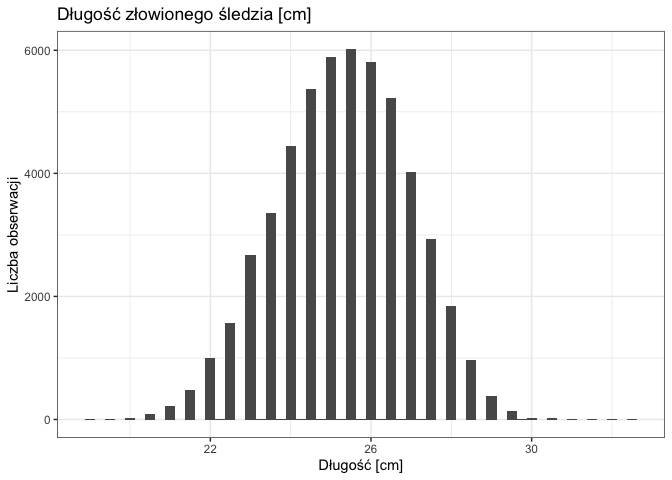
\includegraphics{Project_Herring_Analyze_files/figure-latex/cechy1-1.pdf}
Jak możemy zaobserwować, większość śledzi w połowie ma długość od 23 do
27 centymetrów.

\begin{Shaded}
\begin{Highlighting}[]
\NormalTok{plot_cfin1 <-}\StringTok{ }\KeywordTok{ggplot}\NormalTok{(content, }\KeywordTok{aes}\NormalTok{(}\DataTypeTok{x =}\NormalTok{ cfin1)) }\OperatorTok{+}\StringTok{ }\KeywordTok{geom_histogram}\NormalTok{(}\DataTypeTok{binwidth =} \FloatTok{1.0}\NormalTok{) }\OperatorTok{+}
\StringTok{  }\KeywordTok{theme_bw}\NormalTok{() }\OperatorTok{+}\StringTok{ }\KeywordTok{ggtitle}\NormalTok{(}\StringTok{'Calanus finmarchicus gat. 1'}\NormalTok{) }\OperatorTok{+}\StringTok{ }
\StringTok{  }\KeywordTok{xlab}\NormalTok{(}\KeywordTok{sprintf}\NormalTok{(}\StringTok{'Zagęszczenie planktonu [j]'}\NormalTok{)) }\OperatorTok{+}\StringTok{ }\KeywordTok{ylab}\NormalTok{(}\StringTok{'Liczba obserwacji'}\NormalTok{)}

\NormalTok{plot_cfin2 <-}\StringTok{ }\KeywordTok{ggplot}\NormalTok{(content, }\KeywordTok{aes}\NormalTok{(}\DataTypeTok{x =}\NormalTok{ cfin2)) }\OperatorTok{+}\StringTok{ }\KeywordTok{geom_histogram}\NormalTok{(}\DataTypeTok{binwidth =} \FloatTok{1.0}\NormalTok{) }\OperatorTok{+}
\StringTok{  }\KeywordTok{theme_bw}\NormalTok{() }\OperatorTok{+}\StringTok{ }\KeywordTok{ggtitle}\NormalTok{(}\StringTok{'Calanus finmarchicus gat. 2'}\NormalTok{) }\OperatorTok{+}\StringTok{ }
\StringTok{  }\KeywordTok{xlab}\NormalTok{(}\KeywordTok{sprintf}\NormalTok{(}\StringTok{'Zagęszczenie planktonu [j]'}\NormalTok{)) }\OperatorTok{+}\StringTok{ }\KeywordTok{ylab}\NormalTok{(}\StringTok{'Liczba obserwacji'}\NormalTok{)}

\KeywordTok{grid.arrange}\NormalTok{(plot_cfin1, plot_cfin2, }\DataTypeTok{nrow =} \DecValTok{1}\NormalTok{)}
\end{Highlighting}
\end{Shaded}

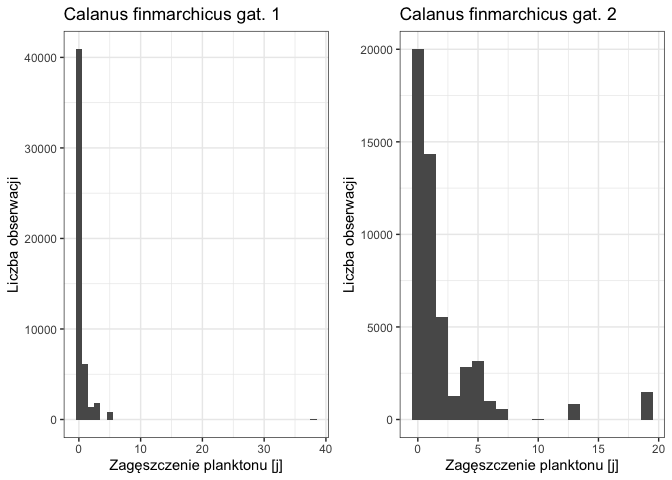
\includegraphics{Project_Herring_Analyze_files/figure-latex/cechy2-1.pdf}

\begin{Shaded}
\begin{Highlighting}[]
\NormalTok{plot_chel1 <-}\StringTok{ }\KeywordTok{ggplot}\NormalTok{(content, }\KeywordTok{aes}\NormalTok{(}\DataTypeTok{x =}\NormalTok{ chel1)) }\OperatorTok{+}\StringTok{ }\KeywordTok{geom_histogram}\NormalTok{(}\DataTypeTok{binwidth =} \FloatTok{0.5}\NormalTok{) }\OperatorTok{+}
\StringTok{  }\KeywordTok{theme_bw}\NormalTok{() }\OperatorTok{+}\StringTok{ }\KeywordTok{ggtitle}\NormalTok{(}\StringTok{'Calanus helgolandicus gat. 1'}\NormalTok{) }\OperatorTok{+}\StringTok{ }
\StringTok{  }\KeywordTok{xlab}\NormalTok{(}\KeywordTok{sprintf}\NormalTok{(}\StringTok{'Zagęszczenie planktonu [j]'}\NormalTok{)) }\OperatorTok{+}\StringTok{ }\KeywordTok{ylab}\NormalTok{(}\StringTok{'Liczba obserwacji'}\NormalTok{)}

\NormalTok{plot_chel2 <-}\StringTok{ }\KeywordTok{ggplot}\NormalTok{(content, }\KeywordTok{aes}\NormalTok{(}\DataTypeTok{x =}\NormalTok{ chel2)) }\OperatorTok{+}\StringTok{ }\KeywordTok{geom_histogram}\NormalTok{(}\DataTypeTok{binwidth =} \FloatTok{0.5}\NormalTok{) }\OperatorTok{+}
\StringTok{  }\KeywordTok{theme_bw}\NormalTok{() }\OperatorTok{+}\StringTok{ }\KeywordTok{ggtitle}\NormalTok{(}\StringTok{'Calanus helgolandicus gat. 2'}\NormalTok{) }\OperatorTok{+}\StringTok{ }
\StringTok{  }\KeywordTok{xlab}\NormalTok{(}\KeywordTok{sprintf}\NormalTok{(}\StringTok{'Zagęszczenie planktonu [j]'}\NormalTok{)) }\OperatorTok{+}\StringTok{ }\KeywordTok{ylab}\NormalTok{(}\StringTok{'Liczba obserwacji'}\NormalTok{)}

\KeywordTok{grid.arrange}\NormalTok{(plot_chel1, plot_chel2, }\DataTypeTok{nrow =} \DecValTok{1}\NormalTok{)}
\end{Highlighting}
\end{Shaded}

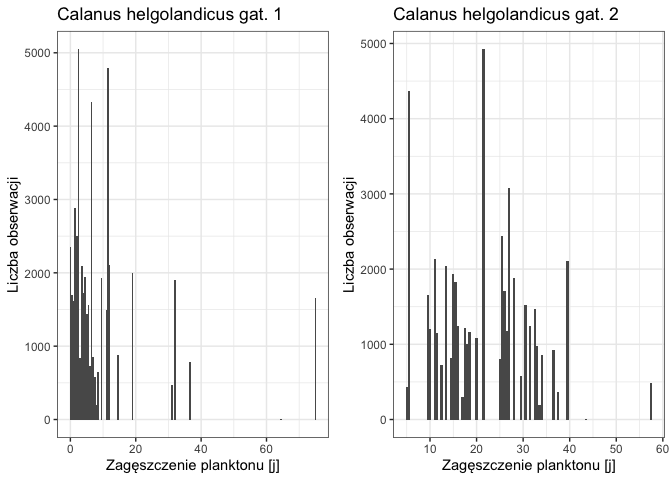
\includegraphics{Project_Herring_Analyze_files/figure-latex/cechy3-1.pdf}

\begin{Shaded}
\begin{Highlighting}[]
\NormalTok{plot_lcop1 <-}\StringTok{ }\KeywordTok{ggplot}\NormalTok{(content, }\KeywordTok{aes}\NormalTok{(}\DataTypeTok{x =}\NormalTok{ lcop1)) }\OperatorTok{+}\StringTok{ }\KeywordTok{geom_histogram}\NormalTok{(}\DataTypeTok{binwidth =} \FloatTok{0.5}\NormalTok{) }\OperatorTok{+}
\StringTok{  }\KeywordTok{theme_bw}\NormalTok{() }\OperatorTok{+}\StringTok{ }\KeywordTok{ggtitle}\NormalTok{(}\StringTok{'Widłonogi gat. 1'}\NormalTok{) }\OperatorTok{+}\StringTok{ }
\StringTok{  }\KeywordTok{xlab}\NormalTok{(}\KeywordTok{sprintf}\NormalTok{(}\StringTok{'Zagęszczenie planktonu [j]'}\NormalTok{)) }\OperatorTok{+}\StringTok{ }\KeywordTok{ylab}\NormalTok{(}\StringTok{'Liczba obserwacji'}\NormalTok{)}

\NormalTok{plot_lcop2 <-}\StringTok{ }\KeywordTok{ggplot}\NormalTok{(content, }\KeywordTok{aes}\NormalTok{(}\DataTypeTok{x =}\NormalTok{ lcop2)) }\OperatorTok{+}\StringTok{ }\KeywordTok{geom_histogram}\NormalTok{(}\DataTypeTok{binwidth =} \FloatTok{0.5}\NormalTok{) }\OperatorTok{+}
\StringTok{  }\KeywordTok{theme_bw}\NormalTok{() }\OperatorTok{+}\StringTok{ }\KeywordTok{ggtitle}\NormalTok{(}\StringTok{'Widłonogi gat. 2'}\NormalTok{) }\OperatorTok{+}\StringTok{ }
\StringTok{  }\KeywordTok{xlab}\NormalTok{(}\KeywordTok{sprintf}\NormalTok{(}\StringTok{'Zagęszczenie planktonu [j]'}\NormalTok{)) }\OperatorTok{+}\StringTok{ }\KeywordTok{ylab}\NormalTok{(}\StringTok{'Liczba obserwacji'}\NormalTok{)}

\KeywordTok{grid.arrange}\NormalTok{(plot_lcop1, plot_lcop2, }\DataTypeTok{nrow =} \DecValTok{1}\NormalTok{)}
\end{Highlighting}
\end{Shaded}

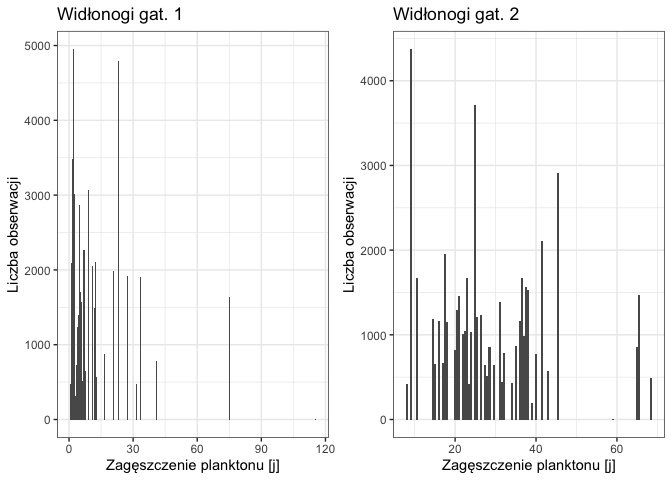
\includegraphics{Project_Herring_Analyze_files/figure-latex/cechy4-1.pdf}

\begin{Shaded}
\begin{Highlighting}[]
\NormalTok{plot_fbar <-}\StringTok{ }\KeywordTok{ggplot}\NormalTok{(content, }\KeywordTok{aes}\NormalTok{(}\DataTypeTok{x =}\NormalTok{ fbar)) }\OperatorTok{+}\StringTok{ }\KeywordTok{geom_histogram}\NormalTok{(}\DataTypeTok{binwidth =} \FloatTok{0.05}\NormalTok{) }\OperatorTok{+}
\StringTok{  }\KeywordTok{theme_bw}\NormalTok{() }\OperatorTok{+}\StringTok{ }\KeywordTok{ggtitle}\NormalTok{(}\StringTok{'Natężenie połowów') + }
\StringTok{  xlab(sprintf('}\NormalTok{Ułamek pozostawionego narybku}\StringTok{')) + ylab('}\NormalTok{Liczba obserwacji}\StringTok{')}

\StringTok{plot_recr <- ggplot(content, aes(x = recr)) + geom_histogram(binwidth = 50000.0) +}
\StringTok{  theme_bw() + ggtitle('}\NormalTok{Roczny narybek}\StringTok{') + }
\StringTok{  xlab(sprintf('}\NormalTok{Liczba śledzi}\StringTok{')) + ylab('}\NormalTok{Liczba obserwacji}\StringTok{')}

\StringTok{plot_cumf <- ggplot(content, aes(x = cumf)) + geom_histogram(binwidth = 0.02) +}
\StringTok{  theme_bw() + ggtitle('}\NormalTok{Łączne roczne natężenie połowów') }\OperatorTok{+}\StringTok{ }
\StringTok{  }\KeywordTok{xlab}\NormalTok{(}\KeywordTok{sprintf}\NormalTok{(}\StringTok{'Ułamek pozostawionego narybku'}\NormalTok{)) }\OperatorTok{+}\StringTok{ }\KeywordTok{ylab}\NormalTok{(}\StringTok{'Liczba obserwacji'}\NormalTok{)}

\NormalTok{plot_totaln <-}\StringTok{ }\KeywordTok{ggplot}\NormalTok{(content, }\KeywordTok{aes}\NormalTok{(}\DataTypeTok{x =}\NormalTok{ totaln)) }\OperatorTok{+}\StringTok{ }\KeywordTok{geom_histogram}\NormalTok{(}\DataTypeTok{binwidth =} \FloatTok{1000.0}\NormalTok{) }\OperatorTok{+}
\StringTok{  }\KeywordTok{theme_bw}\NormalTok{() }\OperatorTok{+}\StringTok{ }\KeywordTok{ggtitle}\NormalTok{(}\StringTok{'Łączna liczba złowionych ryb'}\NormalTok{) }\OperatorTok{+}\StringTok{ }
\StringTok{  }\KeywordTok{xlab}\NormalTok{(}\KeywordTok{sprintf}\NormalTok{(}\StringTok{'Liczba śledzi'}\NormalTok{)) }\OperatorTok{+}\StringTok{ }\KeywordTok{ylab}\NormalTok{(}\StringTok{'Liczba obserwacji'}\NormalTok{)}

\KeywordTok{grid.arrange}\NormalTok{(plot_fbar, plot_recr, plot_cumf, plot_totaln, }\DataTypeTok{nrow =} \DecValTok{2}\NormalTok{)}
\end{Highlighting}
\end{Shaded}

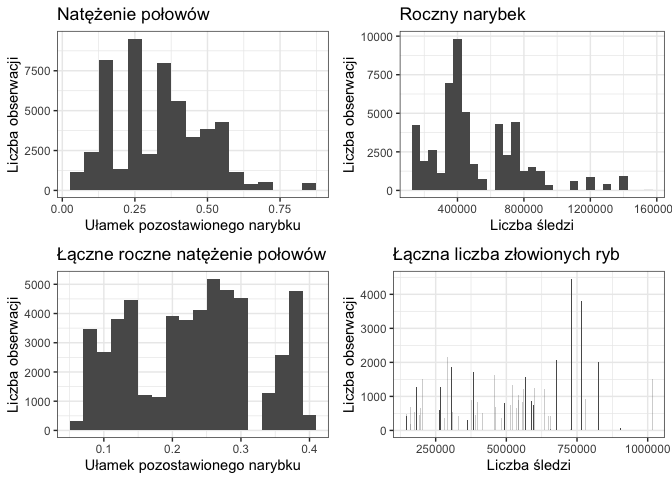
\includegraphics{Project_Herring_Analyze_files/figure-latex/cechy5-1.pdf}

\begin{Shaded}
\begin{Highlighting}[]
\NormalTok{plot_sst <-}\StringTok{ }\KeywordTok{ggplot}\NormalTok{(content, }\KeywordTok{aes}\NormalTok{(}\DataTypeTok{x =}\NormalTok{ sst)) }\OperatorTok{+}\StringTok{ }\KeywordTok{geom_histogram}\NormalTok{(}\DataTypeTok{binwidth =} \FloatTok{0.1}\NormalTok{) }\OperatorTok{+}
\StringTok{  }\KeywordTok{theme_bw}\NormalTok{() }\OperatorTok{+}\StringTok{ }\KeywordTok{ggtitle}\NormalTok{(}\StringTok{'Temperatura przy powierzchni wody'}\NormalTok{) }\OperatorTok{+}\StringTok{ }
\StringTok{  }\KeywordTok{xlab}\NormalTok{(}\KeywordTok{sprintf}\NormalTok{(}\StringTok{'Temperatura'}\NormalTok{)) }\OperatorTok{+}\StringTok{ }\KeywordTok{ylab}\NormalTok{(}\StringTok{'Liczba obserwacji'}\NormalTok{)}

\NormalTok{plot_sal <-}\StringTok{ }\KeywordTok{ggplot}\NormalTok{(content, }\KeywordTok{aes}\NormalTok{(}\DataTypeTok{x =}\NormalTok{ sal)) }\OperatorTok{+}\StringTok{ }\KeywordTok{geom_histogram}\NormalTok{(}\DataTypeTok{binwidth =} \FloatTok{0.01}\NormalTok{) }\OperatorTok{+}
\StringTok{  }\KeywordTok{theme_bw}\NormalTok{() }\OperatorTok{+}\StringTok{ }\KeywordTok{ggtitle}\NormalTok{(}\StringTok{'Poziom zasolenia wody'}\NormalTok{) }\OperatorTok{+}\StringTok{ }
\StringTok{  }\KeywordTok{xlab}\NormalTok{(}\KeywordTok{sprintf}\NormalTok{(}\StringTok{'Zasolenie wody'}\NormalTok{)) }\OperatorTok{+}\StringTok{ }\KeywordTok{ylab}\NormalTok{(}\StringTok{'Liczba obserwacji'}\NormalTok{)}

\NormalTok{plot_xmonth <-}\StringTok{ }\KeywordTok{ggplot}\NormalTok{(content, }\KeywordTok{aes}\NormalTok{(}\DataTypeTok{x =}\NormalTok{ xmonth)) }\OperatorTok{+}\StringTok{ }\KeywordTok{geom_histogram}\NormalTok{(}\DataTypeTok{binwidth =} \FloatTok{0.5}\NormalTok{) }\OperatorTok{+}
\StringTok{  }\KeywordTok{theme_bw}\NormalTok{() }\OperatorTok{+}\StringTok{ }\KeywordTok{ggtitle}\NormalTok{(}\StringTok{'Miesic połowu'}\NormalTok{) }\OperatorTok{+}\StringTok{ }
\StringTok{  }\KeywordTok{xlab}\NormalTok{(}\KeywordTok{sprintf}\NormalTok{(}\StringTok{'Miesiąc'}\NormalTok{)) }\OperatorTok{+}\StringTok{ }\KeywordTok{ylab}\NormalTok{(}\StringTok{'Liczba obserwacji'}\NormalTok{)}

\NormalTok{plot_nao <-}\StringTok{ }\KeywordTok{ggplot}\NormalTok{(content, }\KeywordTok{aes}\NormalTok{(}\DataTypeTok{x =}\NormalTok{ nao)) }\OperatorTok{+}\StringTok{ }\KeywordTok{geom_histogram}\NormalTok{(}\DataTypeTok{binwidth =} \FloatTok{0.5}\NormalTok{) }\OperatorTok{+}
\StringTok{  }\KeywordTok{theme_bw}\NormalTok{() }\OperatorTok{+}\StringTok{ }\KeywordTok{ggtitle}\NormalTok{(}\StringTok{'Oscylacja północnoatlantycka'}\NormalTok{) }\OperatorTok{+}\StringTok{ }
\StringTok{  }\KeywordTok{xlab}\NormalTok{(}\KeywordTok{sprintf}\NormalTok{(}\StringTok{'Oscylacja'}\NormalTok{)) }\OperatorTok{+}\StringTok{ }\KeywordTok{ylab}\NormalTok{(}\StringTok{'Liczba obserwacji'}\NormalTok{)}

\KeywordTok{grid.arrange}\NormalTok{(plot_sst, plot_sal, plot_xmonth, plot_nao, }\DataTypeTok{nrow =} \DecValTok{2}\NormalTok{)}
\end{Highlighting}
\end{Shaded}

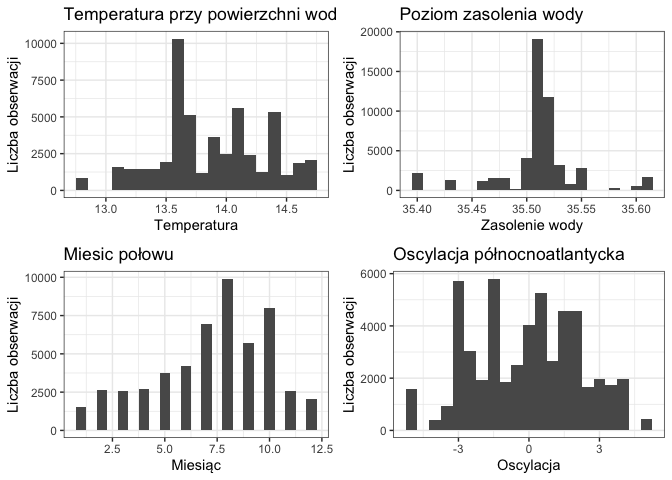
\includegraphics{Project_Herring_Analyze_files/figure-latex/cechy6-1.pdf}

Analizując przedstawione wykresy dotyczące poszczególnych atrybutów
opisujących połowy możemy zaobserwować rozkład zbliżony do normalnego
dla wielu z nich (chociażby parametr długości śledzia). W przypadku
parametrów dostępności planktonu \emph{Calanus finmarchicus gat. 1} oraz
\emph{Widłonogów gat. 1} obserwujemy występowanie drobnej próbki danych
odbierających znacząco od reszty. Na potrzeby dalszego przetwarzania
dane zostaną oczyszczone z tych obserwacji odstających.

TODO: Można opisać pozostałe wykresy bazując na danych w tabeli
poprzedniej (min, max \ldots{})

\begin{Shaded}
\begin{Highlighting}[]
\NormalTok{without_outliers =}
\StringTok{  }\NormalTok{content }\OperatorTok
\StringTok{  }\KeywordTok{filter}\NormalTok{(cfin1 }\OperatorTok{<=}\StringTok{ }\DecValTok{10} \OperatorTok{|}\StringTok{ }\KeywordTok{is.na}\NormalTok{(cfin1)) }\OperatorTok
\StringTok{  }\KeywordTok{filter}\NormalTok{(lcop1 }\OperatorTok{<=}\StringTok{ }\DecValTok{90} \OperatorTok{|}\StringTok{ }\KeywordTok{is.na}\NormalTok{(lcop1))}
\end{Highlighting}
\end{Shaded}

Po operacji w zbiorze obserwacji pozostało 52576 próbek (usunięto 6
obserwacji).

\begin{Shaded}
\begin{Highlighting}[]
\NormalTok{plot_cfin1_clear <-}\StringTok{ }\KeywordTok{ggplot}\NormalTok{(without_outliers, }\KeywordTok{aes}\NormalTok{(}\DataTypeTok{x =}\NormalTok{ cfin1)) }\OperatorTok{+}\StringTok{ }\KeywordTok{geom_histogram}\NormalTok{(}\DataTypeTok{binwidth =} \FloatTok{1.0}\NormalTok{) }\OperatorTok{+}
\StringTok{  }\KeywordTok{theme_bw}\NormalTok{() }\OperatorTok{+}\StringTok{ }\KeywordTok{ggtitle}\NormalTok{(}\StringTok{'Calanus finmarchicus gat. 1'}\NormalTok{) }\OperatorTok{+}\StringTok{ }
\StringTok{  }\KeywordTok{xlab}\NormalTok{(}\KeywordTok{sprintf}\NormalTok{(}\StringTok{'Zagęszczenie planktonu [j]'}\NormalTok{)) }\OperatorTok{+}\StringTok{ }\KeywordTok{ylab}\NormalTok{(}\StringTok{'Liczba obserwacji'}\NormalTok{)}

\NormalTok{plot_lcop1_clear <-}\StringTok{ }\KeywordTok{ggplot}\NormalTok{(without_outliers, }\KeywordTok{aes}\NormalTok{(}\DataTypeTok{x =}\NormalTok{ lcop1)) }\OperatorTok{+}\StringTok{ }\KeywordTok{geom_histogram}\NormalTok{(}\DataTypeTok{binwidth =} \FloatTok{0.5}\NormalTok{) }\OperatorTok{+}
\StringTok{  }\KeywordTok{theme_bw}\NormalTok{() }\OperatorTok{+}\StringTok{ }\KeywordTok{ggtitle}\NormalTok{(}\StringTok{'Widłonogi gat. 1'}\NormalTok{) }\OperatorTok{+}\StringTok{ }
\StringTok{  }\KeywordTok{xlab}\NormalTok{(}\KeywordTok{sprintf}\NormalTok{(}\StringTok{'Zagęszczenie planktonu [j]'}\NormalTok{)) }\OperatorTok{+}\StringTok{ }\KeywordTok{ylab}\NormalTok{(}\StringTok{'Liczba obserwacji'}\NormalTok{)}

\KeywordTok{grid.arrange}\NormalTok{(plot_cfin1_clear, plot_lcop1_clear, }\DataTypeTok{nrow =} \DecValTok{1}\NormalTok{)}
\end{Highlighting}
\end{Shaded}

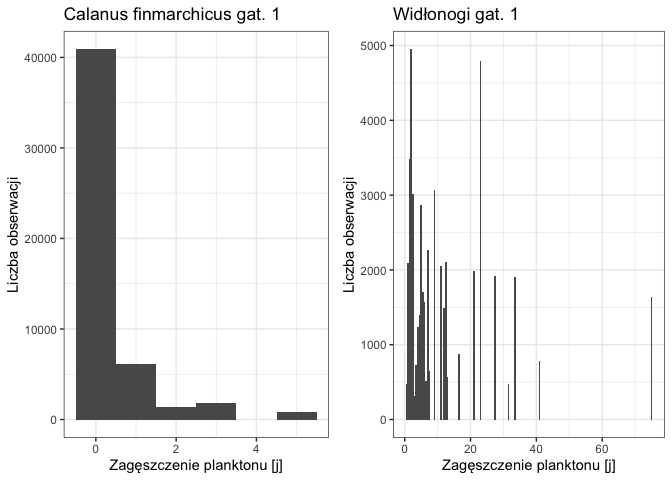
\includegraphics{Project_Herring_Analyze_files/figure-latex/cechy7-1.pdf}

\hypertarget{przetwarzanie-brakujux105cych-danych}{%
\section{Przetwarzanie brakujących
danych}\label{przetwarzanie-brakujux105cych-danych}}

Korzystajac z pakietu \texttt{imputeTS} i funkcji \texttt{statsNA}
możemy przeprowadzić analizę wartości pustych w poszczególnych
obserwacjach.

\begin{Shaded}
\begin{Highlighting}[]
\KeywordTok{library}\NormalTok{(}\StringTok{'imputeTS'}\NormalTok{)}

\NormalTok{without_outliers }\OperatorTok
\StringTok{  }\KeywordTok{colnames}\NormalTok{() }\OperatorTok
\StringTok{  }\KeywordTok{sapply}\NormalTok{(}\ControlFlowTok{function}\NormalTok{(attr) \{}
    \KeywordTok{statsNA}\NormalTok{(without_outliers[[attr]], }\DataTypeTok{printOnly =} \OtherTok{FALSE}\NormalTok{)}
\NormalTok{  \}) }\OperatorTok
\StringTok{  }\KeywordTok{kable}\NormalTok{()}
\end{Highlighting}
\end{Shaded}

\begin{longtable}[]{@{}llllllllllllllll@{}}
\toprule
& length & cfin1 & cfin2 & chel1 & chel2 & lcop1 & lcop2 & fbar & recr &
cumf & totaln & sst & sal & xmonth & nao\tabularnewline
\midrule
\endhead
lengthTimeSeries & 52576 & 52576 & 52576 & 52576 & 52576 & 52576 & 52576
& 52576 & 52576 & 52576 & 52576 & 52576 & 52576 & 52576 &
52576\tabularnewline
numberNAs & 0 & 1581 & 1536 & 1555 & 1556 & 1653 & 1591 & 0 & 0 & 0 & 0
& 1584 & 0 & 0 & 0\tabularnewline
percentageNAs & 0\% & 3.01\% & 2.92\% & 2.96\% & 2.96\% & 3.14\% &
3.03\% & 0\% & 0\% & 0\% & 0\% & 3.01\% & 0\% & 0\% & 0\%\tabularnewline
naGapLongest & NA & 3 & 3 & 3 & 3 & 2 & 3 & NA & NA & NA & NA & 3 & NA &
NA & NA\tabularnewline
naGapMostFrequent & 52576 & 1 & 1 & 1 & 1 & 1 & 1 & 52576 & 52576 &
52576 & 52576 & 1 & 52576 & 52576 & 52576\tabularnewline
naGapMostOverallNAs & 52576 & 1 & 1 & 1 & 1 & 1 & 1 & 52576 & 52576 &
52576 & 52576 & 1 & 52576 & 52576 & 52576\tabularnewline
\bottomrule
\end{longtable}

TODO: Poprawić tabelkę, źle wygląda w PDF

Analizując zaprezentowane podsumowania dla wszystkich atrybutów, możemy
zauważyć że wartości puste stanowią mniej niż 3.5\% całego zbioru
obserwacji. Ponadto ich rozkład ma charater losowy oraz są równomierne.
W danych nie występują długie serie wartości pustych (sekwencje liczące
dwie oraz trzy wartości puste są rzadkie). Wykorzystując wiedzę o
charakterystyce danych możemy wykonać interpolację z wykorzystaniem
filtru Kalmana, aby pozbyć się wartości pustych.

\begin{Shaded}
\begin{Highlighting}[]
\NormalTok{without_outliers}\OperatorTok{$}\NormalTok{cfin1 <-}\StringTok{ }\KeywordTok{na_kalman}\NormalTok{(without_outliers}\OperatorTok{$}\NormalTok{cfin1)}
\NormalTok{without_outliers}\OperatorTok{$}\NormalTok{cfin2 <-}\StringTok{ }\KeywordTok{na_kalman}\NormalTok{(without_outliers}\OperatorTok{$}\NormalTok{cfin2)}
\NormalTok{without_outliers}\OperatorTok{$}\NormalTok{chel1 <-}\StringTok{ }\KeywordTok{na_kalman}\NormalTok{(without_outliers}\OperatorTok{$}\NormalTok{chel1)}
\NormalTok{without_outliers}\OperatorTok{$}\NormalTok{chel2 <-}\StringTok{ }\KeywordTok{na_kalman}\NormalTok{(without_outliers}\OperatorTok{$}\NormalTok{chel2)}
\NormalTok{without_outliers}\OperatorTok{$}\NormalTok{lcop1 <-}\StringTok{ }\KeywordTok{na_kalman}\NormalTok{(without_outliers}\OperatorTok{$}\NormalTok{lcop1)}
\NormalTok{without_outliers}\OperatorTok{$}\NormalTok{lcop2 <-}\StringTok{ }\KeywordTok{na_kalman}\NormalTok{(without_outliers}\OperatorTok{$}\NormalTok{lcop2)}
\NormalTok{without_outliers}\OperatorTok{$}\NormalTok{sst <-}\StringTok{ }\KeywordTok{na_kalman}\NormalTok{(without_outliers}\OperatorTok{$}\NormalTok{sst)}
\end{Highlighting}
\end{Shaded}

TODO: Użyć jakieś funkcji

\hypertarget{korelacja-atrybutuxf3w}{%
\section{Korelacja atrybutów}\label{korelacja-atrybutuxf3w}}

\begin{Shaded}
\begin{Highlighting}[]
\KeywordTok{library}\NormalTok{(}\StringTok{'corrplot'}\NormalTok{)}

\NormalTok{corelation_matrix <-}\StringTok{ }\KeywordTok{cor}\NormalTok{(without_outliers)}
\KeywordTok{corrplot}\NormalTok{(corelation_matrix, }\DataTypeTok{method =} \StringTok{"circle"}\NormalTok{, }\DataTypeTok{title =} \StringTok{"Macierz korelacji"}\NormalTok{)}
\end{Highlighting}
\end{Shaded}

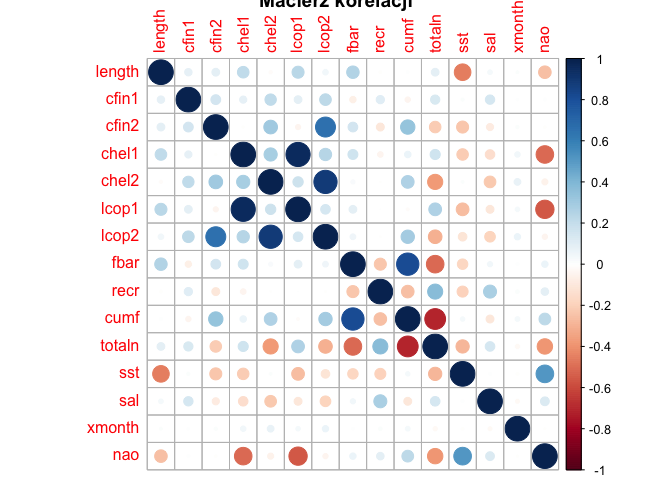
\includegraphics{Project_Herring_Analyze_files/figure-latex/korelacja-1.pdf}

Na wykresie powyższym została przedstawiona macierz korelacji pomiędzy
poszczególnymi atrybutami. Jak możemy zaobserwować, istnieje bardzo
silna pozytywna korelacja pomiędzy parametrem \texttt{chel1} oraz
\texttt{lcop1} (wynosząca w przybliżeniu \texttt{0.96}), a także
\texttt{chel2} oraz \texttt{lcop2} (wynosząca \texttt{0.88}). Wynika z
tego że występowanie planktonu \texttt{Calanus\ helgolandicus\ gat.\ 1}
związane jest z obecnością \texttt{widłonogów\ gat.\ 1} i vice versa.
Podobnie w przypadku planktonów drugiego gatunku czyli pary
\texttt{Calanus\ helgolandicus\ gat.\ 2} oraz
\texttt{widłonogi\ gat.\ 2}.

Analizując dalej macierz korelacji możemy zaobserwować pozytywną
zależność pomiędzy \texttt{cfin2} i \texttt{lcop2} wynosząca
\texttt{0.65} - zagęszczenie \texttt{Calanus\ finmarchicus\ gat.\ 2} ma
powiązanie w obecności \texttt{widłonogów\ gat.\ 2}.

Ciekawą zależnością jest \texttt{sst} oraz \texttt{nao}. Korzystając z
opisu \texttt{oscylacji\ północnoatlantyckiej} na stronie encyklopedii
\href{https://pl.wikipedia.org/wiki/Oscylacja_p\%C3\%B3\%C5\%82nocnoatlantycka}{Wikipedia}
mamy do czynienia ze zjawiskiem meterologicznym wpływającym na klimat,
co manifestuje się między innymi zmianą temperatury. Podkreśla to
wiarygodność naszych obserwacji, gdyż doszło do odwzorowania zjawiska
fizycznego w naszych danych.

Wysoką wartość zależności \texttt{fbar} oznaczającej
\texttt{natężenia\ połowów\ w\ regionie} oraz \texttt{cumf} czyli
\texttt{łączne\ roczne\ natężenie\ połowów\ w\ regionie} wynoszącej
\texttt{0.82} można łatwo wyjaśnić. Łowienie w danym miejscu przez długi
czas sumarycznie wpłynie na wysoką wartość drugiego parametru.

Interesującą z punktu widzenia tematu raportu jest zależność temperatury
przy powierzchni wody i długości złowionego śledzia. Wynosi ona
\texttt{-0.45}. Większa temperatura ma odzwierciedlenie w mniejszych
rozmiarach śledzi.

TODO: Dodać wykresy dla porównań TODO: Poprawić ten opis aby dać tekst a
nie same nazwy kolumn

\hypertarget{zmiennoux15bux107-cech-w-ramach-nastux119pujux105cych-po-siebie-poux142owuxf3w}{%
\section{Zmienność cech w ramach następujących po siebie
połowów}\label{zmiennoux15bux107-cech-w-ramach-nastux119pujux105cych-po-siebie-poux142owuxf3w}}

W kolejnych podrozdziałach zostanie przeanalizowana zmienność cech.
Naszym celem jest wykrycie przyczyny spadku długości śledzi w połowach.

\hypertarget{dux142ugoux15bux107-ux15bledzi}{%
\subsection{Długość śledzi}\label{dux142ugoux15bux107-ux15bledzi}}

\begin{Shaded}
\begin{Highlighting}[]
\NormalTok{df_with_ids <-}\StringTok{ }\KeywordTok{mutate}\NormalTok{(without_outliers, }\DataTypeTok{id =} \KeywordTok{as.numeric}\NormalTok{(}\KeywordTok{rownames}\NormalTok{(without_outliers)))}
\NormalTok{sampled_data <-}\StringTok{ }\KeywordTok{sample_n}\NormalTok{(df_with_ids, }\DecValTok{500}\NormalTok{)}
\end{Highlighting}
\end{Shaded}

\begin{Shaded}
\begin{Highlighting}[]
\NormalTok{zmiana_sledzi_plot <-}\StringTok{ }\KeywordTok{ggplot}\NormalTok{(}
\NormalTok{  sampled_data,}
  \KeywordTok{aes}\NormalTok{(}\DataTypeTok{x=}\NormalTok{id, }\DataTypeTok{y=}\NormalTok{length)}
\NormalTok{) }\OperatorTok{+}\StringTok{ }\KeywordTok{theme_bw}\NormalTok{() }\OperatorTok{+}\StringTok{ }
\StringTok{  }\KeywordTok{theme}\NormalTok{(}\DataTypeTok{axis.text.x=}\KeywordTok{element_blank}\NormalTok{()) }\OperatorTok{+}\StringTok{ }\KeywordTok{geom_point}\NormalTok{() }\OperatorTok{+}\StringTok{ }\KeywordTok{geom_smooth}\NormalTok{(}\DataTypeTok{se =} \OtherTok{FALSE}\NormalTok{, }\DataTypeTok{colour =} \StringTok{"#f5ad00"}\NormalTok{, }\DataTypeTok{size =} \FloatTok{1.0}\NormalTok{) }\OperatorTok{+}\StringTok{ }\KeywordTok{ggtitle}\NormalTok{(}\StringTok{'Zmiana długości śledzia'}\NormalTok{) }\OperatorTok{+}\StringTok{  }\KeywordTok{xlab}\NormalTok{(}\StringTok{''}\NormalTok{) }\OperatorTok{+}\StringTok{ }\KeywordTok{ylab}\NormalTok{(}\StringTok{'Długość [cm]'}\NormalTok{) }\OperatorTok{+}\StringTok{ }\KeywordTok{geom_vline}\NormalTok{(}\DataTypeTok{xintercept =} \DecValTok{17000}\NormalTok{, }\DataTypeTok{colour=}\StringTok{"blue"}\NormalTok{, }\DataTypeTok{linetype =} \DecValTok{2}\NormalTok{, }\DataTypeTok{size =} \FloatTok{1.0}\NormalTok{)}

\NormalTok{zmiana_sledzi_plot}
\end{Highlighting}
\end{Shaded}

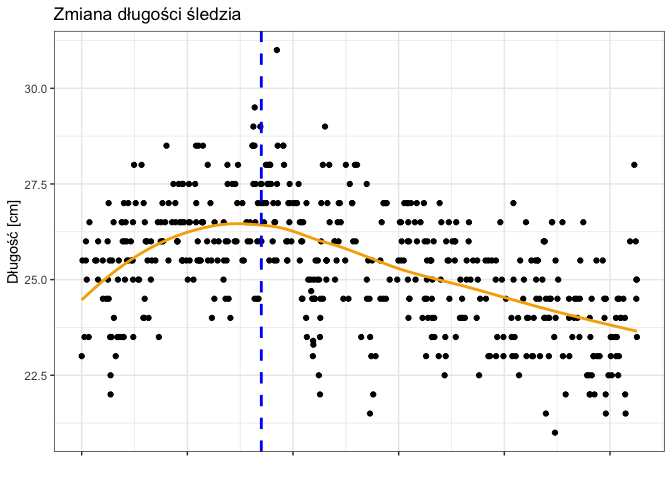
\includegraphics{Project_Herring_Analyze_files/figure-latex/dlugosc-sledzi-1.pdf}

TODO: Opisać wykres

\begin{Shaded}
\begin{Highlighting}[]
\KeywordTok{library}\NormalTok{(}\StringTok{'gganimate'}\NormalTok{)}
\KeywordTok{library}\NormalTok{(}\StringTok{'gifski'}\NormalTok{)}

\KeywordTok{ggplot}\NormalTok{(}
\NormalTok{  sampled_data,}
  \DataTypeTok{group =}\NormalTok{ xmonth,}
  \KeywordTok{aes}\NormalTok{(}\DataTypeTok{x=}\NormalTok{id, }\DataTypeTok{y=}\NormalTok{length)}
\NormalTok{) }\OperatorTok{+}\StringTok{ }\KeywordTok{theme_bw}\NormalTok{() }\OperatorTok{+}\StringTok{ }
\StringTok{  }\KeywordTok{geom_line}\NormalTok{() }\OperatorTok{+}\StringTok{ }\KeywordTok{transition_reveal}\NormalTok{(id)}
\end{Highlighting}
\end{Shaded}

\includegraphics{Project_Herring_Analyze_files/figure-latex/zmiana-rozmiaru-animacja-1.pdf}
\includegraphics{Project_Herring_Analyze_files/figure-latex/zmiana-rozmiaru-animacja-2.pdf}
\includegraphics{Project_Herring_Analyze_files/figure-latex/zmiana-rozmiaru-animacja-3.pdf}
\includegraphics{Project_Herring_Analyze_files/figure-latex/zmiana-rozmiaru-animacja-4.pdf}
\includegraphics{Project_Herring_Analyze_files/figure-latex/zmiana-rozmiaru-animacja-5.pdf}
\includegraphics{Project_Herring_Analyze_files/figure-latex/zmiana-rozmiaru-animacja-6.pdf}
\includegraphics{Project_Herring_Analyze_files/figure-latex/zmiana-rozmiaru-animacja-7.pdf}
\includegraphics{Project_Herring_Analyze_files/figure-latex/zmiana-rozmiaru-animacja-8.pdf}
\includegraphics{Project_Herring_Analyze_files/figure-latex/zmiana-rozmiaru-animacja-9.pdf}
\includegraphics{Project_Herring_Analyze_files/figure-latex/zmiana-rozmiaru-animacja-10.pdf}
\includegraphics{Project_Herring_Analyze_files/figure-latex/zmiana-rozmiaru-animacja-11.pdf}
\includegraphics{Project_Herring_Analyze_files/figure-latex/zmiana-rozmiaru-animacja-12.pdf}
\includegraphics{Project_Herring_Analyze_files/figure-latex/zmiana-rozmiaru-animacja-13.pdf}
\includegraphics{Project_Herring_Analyze_files/figure-latex/zmiana-rozmiaru-animacja-14.pdf}
\includegraphics{Project_Herring_Analyze_files/figure-latex/zmiana-rozmiaru-animacja-15.pdf}
\includegraphics{Project_Herring_Analyze_files/figure-latex/zmiana-rozmiaru-animacja-16.pdf}
\includegraphics{Project_Herring_Analyze_files/figure-latex/zmiana-rozmiaru-animacja-17.pdf}
\includegraphics{Project_Herring_Analyze_files/figure-latex/zmiana-rozmiaru-animacja-18.pdf}
\includegraphics{Project_Herring_Analyze_files/figure-latex/zmiana-rozmiaru-animacja-19.pdf}
\includegraphics{Project_Herring_Analyze_files/figure-latex/zmiana-rozmiaru-animacja-20.pdf}
\includegraphics{Project_Herring_Analyze_files/figure-latex/zmiana-rozmiaru-animacja-21.pdf}
\includegraphics{Project_Herring_Analyze_files/figure-latex/zmiana-rozmiaru-animacja-22.pdf}
\includegraphics{Project_Herring_Analyze_files/figure-latex/zmiana-rozmiaru-animacja-23.pdf}
\includegraphics{Project_Herring_Analyze_files/figure-latex/zmiana-rozmiaru-animacja-24.pdf}
\includegraphics{Project_Herring_Analyze_files/figure-latex/zmiana-rozmiaru-animacja-25.pdf}
\includegraphics{Project_Herring_Analyze_files/figure-latex/zmiana-rozmiaru-animacja-26.pdf}
\includegraphics{Project_Herring_Analyze_files/figure-latex/zmiana-rozmiaru-animacja-27.pdf}
\includegraphics{Project_Herring_Analyze_files/figure-latex/zmiana-rozmiaru-animacja-28.pdf}
\includegraphics{Project_Herring_Analyze_files/figure-latex/zmiana-rozmiaru-animacja-29.pdf}
\includegraphics{Project_Herring_Analyze_files/figure-latex/zmiana-rozmiaru-animacja-30.pdf}
\includegraphics{Project_Herring_Analyze_files/figure-latex/zmiana-rozmiaru-animacja-31.pdf}
\includegraphics{Project_Herring_Analyze_files/figure-latex/zmiana-rozmiaru-animacja-32.pdf}
\includegraphics{Project_Herring_Analyze_files/figure-latex/zmiana-rozmiaru-animacja-33.pdf}
\includegraphics{Project_Herring_Analyze_files/figure-latex/zmiana-rozmiaru-animacja-34.pdf}
\includegraphics{Project_Herring_Analyze_files/figure-latex/zmiana-rozmiaru-animacja-35.pdf}
\includegraphics{Project_Herring_Analyze_files/figure-latex/zmiana-rozmiaru-animacja-36.pdf}
\includegraphics{Project_Herring_Analyze_files/figure-latex/zmiana-rozmiaru-animacja-37.pdf}
\includegraphics{Project_Herring_Analyze_files/figure-latex/zmiana-rozmiaru-animacja-38.pdf}
\includegraphics{Project_Herring_Analyze_files/figure-latex/zmiana-rozmiaru-animacja-39.pdf}
\includegraphics{Project_Herring_Analyze_files/figure-latex/zmiana-rozmiaru-animacja-40.pdf}
\includegraphics{Project_Herring_Analyze_files/figure-latex/zmiana-rozmiaru-animacja-41.pdf}
\includegraphics{Project_Herring_Analyze_files/figure-latex/zmiana-rozmiaru-animacja-42.pdf}
\includegraphics{Project_Herring_Analyze_files/figure-latex/zmiana-rozmiaru-animacja-43.pdf}
\includegraphics{Project_Herring_Analyze_files/figure-latex/zmiana-rozmiaru-animacja-44.pdf}
\includegraphics{Project_Herring_Analyze_files/figure-latex/zmiana-rozmiaru-animacja-45.pdf}
\includegraphics{Project_Herring_Analyze_files/figure-latex/zmiana-rozmiaru-animacja-46.pdf}
\includegraphics{Project_Herring_Analyze_files/figure-latex/zmiana-rozmiaru-animacja-47.pdf}
\includegraphics{Project_Herring_Analyze_files/figure-latex/zmiana-rozmiaru-animacja-48.pdf}
\includegraphics{Project_Herring_Analyze_files/figure-latex/zmiana-rozmiaru-animacja-49.pdf}
\includegraphics{Project_Herring_Analyze_files/figure-latex/zmiana-rozmiaru-animacja-50.pdf}
\includegraphics{Project_Herring_Analyze_files/figure-latex/zmiana-rozmiaru-animacja-51.pdf}
\includegraphics{Project_Herring_Analyze_files/figure-latex/zmiana-rozmiaru-animacja-52.pdf}
\includegraphics{Project_Herring_Analyze_files/figure-latex/zmiana-rozmiaru-animacja-53.pdf}
\includegraphics{Project_Herring_Analyze_files/figure-latex/zmiana-rozmiaru-animacja-54.pdf}
\includegraphics{Project_Herring_Analyze_files/figure-latex/zmiana-rozmiaru-animacja-55.pdf}
\includegraphics{Project_Herring_Analyze_files/figure-latex/zmiana-rozmiaru-animacja-56.pdf}
\includegraphics{Project_Herring_Analyze_files/figure-latex/zmiana-rozmiaru-animacja-57.pdf}
\includegraphics{Project_Herring_Analyze_files/figure-latex/zmiana-rozmiaru-animacja-58.pdf}
\includegraphics{Project_Herring_Analyze_files/figure-latex/zmiana-rozmiaru-animacja-59.pdf}
\includegraphics{Project_Herring_Analyze_files/figure-latex/zmiana-rozmiaru-animacja-60.pdf}
\includegraphics{Project_Herring_Analyze_files/figure-latex/zmiana-rozmiaru-animacja-61.pdf}
\includegraphics{Project_Herring_Analyze_files/figure-latex/zmiana-rozmiaru-animacja-62.pdf}
\includegraphics{Project_Herring_Analyze_files/figure-latex/zmiana-rozmiaru-animacja-63.pdf}
\includegraphics{Project_Herring_Analyze_files/figure-latex/zmiana-rozmiaru-animacja-64.pdf}
\includegraphics{Project_Herring_Analyze_files/figure-latex/zmiana-rozmiaru-animacja-65.pdf}
\includegraphics{Project_Herring_Analyze_files/figure-latex/zmiana-rozmiaru-animacja-66.pdf}
\includegraphics{Project_Herring_Analyze_files/figure-latex/zmiana-rozmiaru-animacja-67.pdf}
\includegraphics{Project_Herring_Analyze_files/figure-latex/zmiana-rozmiaru-animacja-68.pdf}
\includegraphics{Project_Herring_Analyze_files/figure-latex/zmiana-rozmiaru-animacja-69.pdf}
\includegraphics{Project_Herring_Analyze_files/figure-latex/zmiana-rozmiaru-animacja-70.pdf}
\includegraphics{Project_Herring_Analyze_files/figure-latex/zmiana-rozmiaru-animacja-71.pdf}
\includegraphics{Project_Herring_Analyze_files/figure-latex/zmiana-rozmiaru-animacja-72.pdf}
\includegraphics{Project_Herring_Analyze_files/figure-latex/zmiana-rozmiaru-animacja-73.pdf}
\includegraphics{Project_Herring_Analyze_files/figure-latex/zmiana-rozmiaru-animacja-74.pdf}
\includegraphics{Project_Herring_Analyze_files/figure-latex/zmiana-rozmiaru-animacja-75.pdf}
\includegraphics{Project_Herring_Analyze_files/figure-latex/zmiana-rozmiaru-animacja-76.pdf}
\includegraphics{Project_Herring_Analyze_files/figure-latex/zmiana-rozmiaru-animacja-77.pdf}
\includegraphics{Project_Herring_Analyze_files/figure-latex/zmiana-rozmiaru-animacja-78.pdf}
\includegraphics{Project_Herring_Analyze_files/figure-latex/zmiana-rozmiaru-animacja-79.pdf}
\includegraphics{Project_Herring_Analyze_files/figure-latex/zmiana-rozmiaru-animacja-80.pdf}
\includegraphics{Project_Herring_Analyze_files/figure-latex/zmiana-rozmiaru-animacja-81.pdf}
\includegraphics{Project_Herring_Analyze_files/figure-latex/zmiana-rozmiaru-animacja-82.pdf}
\includegraphics{Project_Herring_Analyze_files/figure-latex/zmiana-rozmiaru-animacja-83.pdf}
\includegraphics{Project_Herring_Analyze_files/figure-latex/zmiana-rozmiaru-animacja-84.pdf}
\includegraphics{Project_Herring_Analyze_files/figure-latex/zmiana-rozmiaru-animacja-85.pdf}
\includegraphics{Project_Herring_Analyze_files/figure-latex/zmiana-rozmiaru-animacja-86.pdf}
\includegraphics{Project_Herring_Analyze_files/figure-latex/zmiana-rozmiaru-animacja-87.pdf}
\includegraphics{Project_Herring_Analyze_files/figure-latex/zmiana-rozmiaru-animacja-88.pdf}
\includegraphics{Project_Herring_Analyze_files/figure-latex/zmiana-rozmiaru-animacja-89.pdf}
\includegraphics{Project_Herring_Analyze_files/figure-latex/zmiana-rozmiaru-animacja-90.pdf}
\includegraphics{Project_Herring_Analyze_files/figure-latex/zmiana-rozmiaru-animacja-91.pdf}
\includegraphics{Project_Herring_Analyze_files/figure-latex/zmiana-rozmiaru-animacja-92.pdf}
\includegraphics{Project_Herring_Analyze_files/figure-latex/zmiana-rozmiaru-animacja-93.pdf}
\includegraphics{Project_Herring_Analyze_files/figure-latex/zmiana-rozmiaru-animacja-94.pdf}
\includegraphics{Project_Herring_Analyze_files/figure-latex/zmiana-rozmiaru-animacja-95.pdf}
\includegraphics{Project_Herring_Analyze_files/figure-latex/zmiana-rozmiaru-animacja-96.pdf}
\includegraphics{Project_Herring_Analyze_files/figure-latex/zmiana-rozmiaru-animacja-97.pdf}
\includegraphics{Project_Herring_Analyze_files/figure-latex/zmiana-rozmiaru-animacja-98.pdf}
\includegraphics{Project_Herring_Analyze_files/figure-latex/zmiana-rozmiaru-animacja-99.pdf}
\includegraphics{Project_Herring_Analyze_files/figure-latex/zmiana-rozmiaru-animacja-100.pdf}

TODO: Źródło danych w postaci uśrednionych danych z połowów TODO: Opisać
wykres

\hypertarget{dostux119pnoux15bux107-pokarmu}{%
\subsection{Dostępność pokarmu}\label{dostux119pnoux15bux107-pokarmu}}

\begin{Shaded}
\begin{Highlighting}[]
\KeywordTok{library}\NormalTok{(}\StringTok{'reshape2'}\NormalTok{)}

\NormalTok{plancton_food <-}\StringTok{ }\KeywordTok{melt}\NormalTok{(sampled_data[, }\KeywordTok{c}\NormalTok{(}\DecValTok{16}\NormalTok{, }\DecValTok{2}\OperatorTok{:}\DecValTok{7}\NormalTok{)], }\DataTypeTok{id.vars =} \KeywordTok{c}\NormalTok{(}\StringTok{'id'}\NormalTok{), }\DataTypeTok{variable.name =} \StringTok{"TypPlanktonu"}\NormalTok{, }\DataTypeTok{value.name =} \StringTok{"Values"}\NormalTok{)}
\KeywordTok{ggplot}\NormalTok{(}
\NormalTok{  plancton_food,}
  \KeywordTok{aes}\NormalTok{(id, Values, }\DataTypeTok{color =}\NormalTok{ TypPlanktonu)}
\NormalTok{) }\OperatorTok{+}\StringTok{ }\KeywordTok{theme_bw}\NormalTok{() }\OperatorTok{+}\StringTok{ }
\StringTok{  }\KeywordTok{theme}\NormalTok{(}\DataTypeTok{axis.text.x=}\KeywordTok{element_blank}\NormalTok{()) }\OperatorTok{+}\StringTok{ }\KeywordTok{geom_smooth}\NormalTok{(}\DataTypeTok{se =} \OtherTok{FALSE}\NormalTok{) }\OperatorTok{+}\StringTok{ }\KeywordTok{ggtitle}\NormalTok{(}\StringTok{'Zmiana dostępności pokarmu'}\NormalTok{) }\OperatorTok{+}\StringTok{  }\KeywordTok{xlab}\NormalTok{(}\StringTok{''}\NormalTok{) }\OperatorTok{+}\StringTok{ }\KeywordTok{ylab}\NormalTok{(}\StringTok{'Dostępność pokarmu [zagęszczenie]'}\NormalTok{) }\OperatorTok{+}\StringTok{ }\KeywordTok{geom_vline}\NormalTok{(}\DataTypeTok{xintercept =} \DecValTok{17000}\NormalTok{, }\DataTypeTok{colour=}\StringTok{"blue"}\NormalTok{, }\DataTypeTok{linetype =} \DecValTok{2}\NormalTok{, }\DataTypeTok{size =} \FloatTok{1.0}\NormalTok{)}
\end{Highlighting}
\end{Shaded}

\includegraphics{Project_Herring_Analyze_files/figure-latex/dostepnosc-pokarmu-1.pdf}

TODO: Opisać wykres

\hypertarget{parametry-ux15brodowiska}{%
\subsection{Parametry środowiska}\label{parametry-ux15brodowiska}}

\begin{Shaded}
\begin{Highlighting}[]
\NormalTok{parametry_srodowiska <-}\StringTok{ }\NormalTok{sampled_data[, }\KeywordTok{c}\NormalTok{(}\DecValTok{12}\NormalTok{, }\DecValTok{13}\NormalTok{, }\DecValTok{15}\NormalTok{)]}
\NormalTok{normalized_environment <-}\StringTok{ }\KeywordTok{as.data.frame}\NormalTok{(}\KeywordTok{lapply}\NormalTok{(parametry_srodowiska, }\ControlFlowTok{function}\NormalTok{(x) \{}
\NormalTok{  (x }\OperatorTok{-}\StringTok{ }\KeywordTok{min}\NormalTok{(x)) }\OperatorTok{/}\StringTok{ }\NormalTok{(}\KeywordTok{max}\NormalTok{(x) }\OperatorTok{-}\StringTok{ }\KeywordTok{min}\NormalTok{(x))}
\NormalTok{\}))}
\NormalTok{normalized_environment[}\StringTok{"id"}\NormalTok{] <-}\StringTok{ }\NormalTok{sampled_data[, }\DecValTok{16}\NormalTok{]}

\NormalTok{environment <-}\StringTok{ }\KeywordTok{melt}\NormalTok{(normalized_environment, }\DataTypeTok{id.vars =} \KeywordTok{c}\NormalTok{(}\StringTok{'id'}\NormalTok{), }\DataTypeTok{variable.name =} \StringTok{"Środowisko"}\NormalTok{, }\DataTypeTok{value.name =} \StringTok{"Values"}\NormalTok{)}
\KeywordTok{ggplot}\NormalTok{(}
\NormalTok{  environment,}
  \KeywordTok{aes}\NormalTok{(id, Values, }\DataTypeTok{color =}\NormalTok{ Środowisko)}
\NormalTok{) }\OperatorTok{+}\StringTok{ }\KeywordTok{theme_bw}\NormalTok{() }\OperatorTok{+}\StringTok{ }
\StringTok{  }\KeywordTok{theme}\NormalTok{(}\DataTypeTok{axis.text.x=}\KeywordTok{element_blank}\NormalTok{()) }\OperatorTok{+}\StringTok{ }\KeywordTok{geom_smooth}\NormalTok{(}\DataTypeTok{se =} \OtherTok{FALSE}\NormalTok{) }\OperatorTok{+}\StringTok{ }\KeywordTok{ggtitle}\NormalTok{(}\StringTok{'Zmiana warunków środowiska'}\NormalTok{) }\OperatorTok{+}\StringTok{  }\KeywordTok{xlab}\NormalTok{(}\StringTok{''}\NormalTok{) }\OperatorTok{+}\StringTok{ }\KeywordTok{ylab}\NormalTok{(}\StringTok{'Środowisko (znormalizowana wartość)'}\NormalTok{) }\OperatorTok{+}\StringTok{ }\KeywordTok{geom_vline}\NormalTok{(}\DataTypeTok{xintercept =} \DecValTok{17000}\NormalTok{, }\DataTypeTok{colour=}\StringTok{"blue"}\NormalTok{, }\DataTypeTok{linetype =} \DecValTok{2}\NormalTok{, }\DataTypeTok{size =} \FloatTok{1.0}\NormalTok{)}
\end{Highlighting}
\end{Shaded}

\includegraphics{Project_Herring_Analyze_files/figure-latex/srodowisko-1.pdf}

TODO: Opisać wykres

\hypertarget{eksploatacja-ux142owiska}{%
\subsection{Eksploatacja łowiska}\label{eksploatacja-ux142owiska}}

\begin{Shaded}
\begin{Highlighting}[]
\NormalTok{parametry_lowiska <-}\StringTok{ }\NormalTok{sampled_data[, }\KeywordTok{c}\NormalTok{(}\DecValTok{8}\OperatorTok{:}\DecValTok{11}\NormalTok{)]}
\NormalTok{normalized_lowisko <-}\StringTok{ }\KeywordTok{as.data.frame}\NormalTok{(}\KeywordTok{lapply}\NormalTok{(parametry_lowiska, }\ControlFlowTok{function}\NormalTok{(x) \{}
\NormalTok{  (x }\OperatorTok{-}\StringTok{ }\KeywordTok{min}\NormalTok{(x)) }\OperatorTok{/}\StringTok{ }\NormalTok{(}\KeywordTok{max}\NormalTok{(x) }\OperatorTok{-}\StringTok{ }\KeywordTok{min}\NormalTok{(x))}
\NormalTok{\}))}
\NormalTok{normalized_lowisko[}\StringTok{"id"}\NormalTok{] <-}\StringTok{ }\NormalTok{sampled_data[, }\DecValTok{16}\NormalTok{]}

\NormalTok{lowisko <-}\StringTok{ }\KeywordTok{melt}\NormalTok{(normalized_lowisko, }\DataTypeTok{id.vars =} \KeywordTok{c}\NormalTok{(}\StringTok{'id'}\NormalTok{), }\DataTypeTok{variable.name =} \StringTok{"Łowisko"}\NormalTok{, }\DataTypeTok{value.name =} \StringTok{"Values"}\NormalTok{)}
\KeywordTok{ggplot}\NormalTok{(}
\NormalTok{  lowisko,}
  \KeywordTok{aes}\NormalTok{(id, Values, }\DataTypeTok{color =}\NormalTok{ Łowisko)}
\NormalTok{) }\OperatorTok{+}\StringTok{ }\KeywordTok{theme_bw}\NormalTok{() }\OperatorTok{+}\StringTok{ }
\StringTok{  }\KeywordTok{theme}\NormalTok{(}\DataTypeTok{axis.text.x=}\KeywordTok{element_blank}\NormalTok{()) }\OperatorTok{+}\StringTok{ }\KeywordTok{geom_smooth}\NormalTok{(}\DataTypeTok{se =} \OtherTok{FALSE}\NormalTok{) }\OperatorTok{+}\StringTok{ }\KeywordTok{ggtitle}\NormalTok{(}\StringTok{'Zmiana warunków eksploracji łowiska'}\NormalTok{) }\OperatorTok{+}\StringTok{  }\KeywordTok{xlab}\NormalTok{(}\StringTok{''}\NormalTok{) }\OperatorTok{+}\StringTok{ }\KeywordTok{ylab}\NormalTok{(}\StringTok{'Łowisko (znormalizowana wartość)'}\NormalTok{) }\OperatorTok{+}\StringTok{ }\KeywordTok{geom_vline}\NormalTok{(}\DataTypeTok{xintercept =} \DecValTok{17000}\NormalTok{, }\DataTypeTok{colour=}\StringTok{"blue"}\NormalTok{, }\DataTypeTok{linetype =} \DecValTok{2}\NormalTok{, }\DataTypeTok{size =} \FloatTok{1.0}\NormalTok{)}
\end{Highlighting}
\end{Shaded}

\includegraphics{Project_Herring_Analyze_files/figure-latex/lowisko-1.pdf}

TODO: Opisać wykres

\hypertarget{regresor---predykcja}{%
\section{Regresor - predykcja}\label{regresor---predykcja}}

TODO: Dwa regresory TODO: Wskazanie najważniejszych cech TODO:
Obliczenie błędów


\end{document}
